\documentclass[12pt]{exam}

% \usetikzlibrary{calc,patterns}

\newcommand{\Version}{1} 
\newcommand{\Solutions}{0} 

% TEST SPECIFIC INFORMATION
\ifnum \Version=1 \newcommand{\TestName}{MATH 2552 Participation Activity 4: Pullback Car} \fi


% LOAD PACKAGES
\usepackage{amsmath} % allows for align env and other things
\usepackage{amssymb} % 
\usepackage{mathtools} % allows for single apostrophe
\usepackage{enumitem} % allows for alpha lettering in enumerated lists
\usepackage{lastpage}
\usepackage{array} % for table alignments

\usepackage{graphicx} % if images are needed
\usepackage{wrapfig} % to allow text wrapping

\addpoints

\usepackage{pgfplots} % for surfaces (chapter 7)
\usepackage{tikz-3dplot} 
\pgfplotsset{compat=1.9}
\usetikzlibrary{decorations.pathmorphing,patterns} % for some tikz diagrams
% ~~~~~~~~~~~~~~~~~~~~~~~~~~~~~~~~~~~~
% INITIALS
\newcommand{\Initials}{\textit{\Course, \TestName. Your initials: \underline{\hspace{3cm}}} \vspace{1pt}}

\newcommand{\InitialsLeft}{\noindent \hspace{-18pt}\textit{\Course, \TestName. Your initials: \underline{\hspace{3cm}}} \vspace{1pt}}

\newcommand{\InitialsRight}{\begin{flushright}\textit{\Course, \TestName. Your initials: \underline{\hspace{3cm}}} \vspace{1pt}\end{flushright}}

% ADJUST FIRST LINE IN PARAGRAPH INDENTATION 
\setlength\parindent{0pt}

% FONT FORMAT
\renewcommand*\rmdefault{lmss} % change font to lat mod ss

% ADJUST MARGINS 
\usepackage[a4paper, tmargin=0.8in,bmargin=0.8in,left=1in,right=1in]{geometry}

% TIKZ DIAGRAMS
\usepackage{color}
\usepackage{tikz}  \usetikzlibrary{arrows} 
\usetikzlibrary{calc} 

% COURSE SPECIFIC INFORMATION
\newcommand{\Course}{Math 2552, Differential Equations}
\newcommand{\Instructors}{}

\newcommand{\LastPage}{\begin{center}\textit{This page may be used for scratch work. Please indicate clearly if you would like your work on this page to be graded. }\end{center}   }

% DERIVATIVES
\newcommand{\dfdy}{{\frac{df}{dy}}} % 
\newcommand{\dydt}{{\frac{dy}{dt}}} % 
\newcommand{\dxdt}{{\frac{dx}{dt}}} % 
\newcommand{\dydx}{{\frac{dy}{dx}}} % 
\newcommand{\dydtt}{{\frac{d ^2y}{dt^2}}} % 
\newcommand{\dydxx}{{\frac{d^2y}{dx^2}}} % 
\newcommand{\dydttt}{{\frac{d^3y}{dt^3}}} % 

\newcommand{\ddt}{{\frac{d}{dt}}} % 
\newcommand{\ddx}{{\frac{d}{dx}}} % 
\newcommand{\ddy}{{\frac{d}{dy}}} % 
\newcommand{\dudt}{{\frac{du}{dt}}} % 
\newcommand{\dvdx}{{\frac{dv}{dx}}} % 
\newcommand{\dxdtt}{{\frac{d^2x}{dt^2}}} % 
\newcommand{\dzdt}{{\frac{dz}{dt}}} % 

% COLORS FOR SOLUTIONS
\definecolor{DarkBlue}{rgb}{0.0,0.2,0.4} % 
\definecolor{DarkRed}{rgb}{0.4,0.1,0.1} % 
\definecolor{DarkGreen}{rgb}{0.0,0.25,0.15} % 

% % ADJUST MARGINS
% \usepackage[tmargin=2.0in,bmargin=1.5in]{geometry}
% \geometry{margin=0.76in}

% ADJUST FIRST LINE IN PARAGRAPH INDENTATION 
\setlength\parindent{0pt}

% FONT FORMAT
\renewcommand*\rmdefault{lmss} % change font to lat mod ss


% HEADERS AND FOOTERS
\pagestyle{headandfoot}
\runningfooter{}{}{}
\runningheader{}{}{\textit{\TestName, Page \thepage \ of \pageref{LastPage}} }
% \headheight 42pt % distance from top of page to top of header
% \headsep 12pt % space between header and top of body


\begin{document}
    
\vspace*{-1cm}

\begin{center}
{\Large \TestName}
\end{center}
\newcommand{\ID}{Please print your first name: \framebox{\strut\hspace{4.2cm}}, last name: \framebox{\strut\hspace{4.2cm}}, \\[2pt] and the remaining digits of your GTID:  \framebox{\strut $9$}\framebox{\strut $0$}\framebox{\strut\hspace{0.19cm}}\framebox{\strut\hspace{0.19cm}}\framebox{\strut\hspace{0.19cm}}\framebox{\strut\hspace{0.19cm}}\framebox{\strut\hspace{0.19cm}}\framebox{\strut\hspace{0.19cm}}\framebox{\strut\hspace{0.19cm}}.}

\ID

\vspace{6pt}
\textbf{Instructions}: for full credit please show your work and answer all questions. Your work will be graded for completion, not accuracy. Please submit your work before the end of lecture. 
\subsection*{Pullback Car Dynamics}
A pullback car is a toy with mass $m$ that works as follows. 
    \begin{itemize}
        \item If the car is pulled backwards a short distance along a horizontal surface, and then released from rest at time $t=0$, the car moves forward. 
        \item While the car is moving there are (at least) two forces that are involved:
        
\begin{enumerate}[label=\alph*)]        
        \item The engine of the car pushes the car forward with force $F(t)$. The engine switches off after an unknown amount of time, $t_0$, after the car is released. 
        \item A frictional force pushes the car in the direction opposite of motion. For simplicity, assume that this force is proportional to the velocity of the car. 
    \end{enumerate} 
    \end{itemize}

\begin{center}
    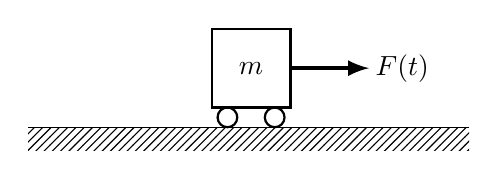
\begin{tikzpicture}
\tikzstyle{spring}=[thick,decorate,decoration={zigzag,pre length=0.3cm,post length=0.3cm,segment length=6}]
\tikzstyle{damper}=[thick,decoration={markings,  
  mark connection node=dmp,
  mark=at position 0.5 with 
  {
    \node (dmp) [thick,inner sep=0pt,transform shape,rotate=-90,minimum width=15pt,minimum height=3pt,draw=none] {};
    \draw [thick] ($(dmp.north east)+(2pt,0)$) -- (dmp.south east) -- (dmp.south west) -- ($(dmp.north west)+(2pt,0)$);
    \draw [thick] ($(dmp.north)+(0,-5pt)$) -- ($(dmp.north)+(0,5pt)$);
  }
}, decorate]

% WALL PATTERN
\tikzstyle{ground}=[fill,pattern=north east lines,draw=none,minimum width=0.75cm,minimum height=0.3cm,inner sep=0pt,outer sep=0pt]

% CART
\node [style={draw,outer sep=0pt,thick}] (M) [minimum width=1cm, minimum height=1.0cm] {$m$};
% WHEELS
\draw [thick] (M.south west) ++ (0.2cm,-0.125cm) circle (0.125cm)  (M.south east) ++ (-0.2cm,-0.125cm) circle (0.125cm);

% BOTTOM GROUND
\node (ground) [ground,anchor=north,yshift=-0.25cm,minimum width=5.6cm,xshift=-0.03cm] at (M.south) {};
\draw (ground.north east) -- (ground.north west);
% \draw (ground.south east) -- (ground.south west);
% \draw (ground.north east) -- (ground.south east);

% % WEST WALL
% \node (wall) [ground, rotate=-90, minimum width=3cm,yshift=-3cm] {};
% \draw (wall.north east) -- (wall.north west);
% \draw (wall.north west) -- (wall.south west);
% \draw (wall.south west) -- (wall.south east);

% SOUTHWEST CORNER WALL
% \node (fill) [ground,xshift=-0.15cm,minimum height = 0.3cm, minimum width = 0.3cm] at (ground.west) {};
% \draw (fill.north west) -- (fill.south west);
% \draw (fill.south west) -- (fill.south east);

% LABEL FOR VECTOR
\node (y) at (M.east) [xshift = 1.42cm] {$F(t)$};
% VECTOR
\draw [-latex,ultra thick] (M.east) ++ (0cm,0cm) -- +(1cm,0cm);

% DAMPER AND SPRING
% \draw [spring] (wall.170) -- ($(M.north west)!(wall.170)!(M.south west)$);
% \draw [damper] (wall.10) -- ($(M.north west)!(wall.10)!(M.south west)$);

\end{tikzpicture}
\end{center}
\subsection*{Questions}
\begin{questions}

% \question[1] Without setting up a DE, draw what you think are the phase portraits for A) the time interval $0 \le t \le t_0$, and B) for $t \ge t_0$. \vspace{12pt}
% \begin{center}
% \begin{tikzpicture}[scale=0.85]
% \draw[help lines] (-.5,-.5) grid (5.5, 5.5);
% \draw[ultra thick, ->] (-1, 0) -- (5.75, 0) ;
% \draw[ultra thick, ->] (0, -1) -- (0, 5.75);
% \node[overlay, above] at (3, 5.75) {A) $0\le t \le t_0$};
% \end{tikzpicture}    \hspace{2cm}    \begin{tikzpicture}[scale=0.85]
% \draw[help lines] (-.5,-.5) grid (5.5, 5.5);
% \draw[ultra thick, ->] (-1, 0) -- (5.75, 0) ;
% \draw[ultra thick, ->] (0, -1) -- (0, 5.75);
% \node[overlay, above] at (3, 5.75) {B) $t \ge t_0$};
% \end{tikzpicture}
% \end{center}
% \newpage
\question[1] Construct DEs that model the car motion for A) $0\le t \le t_0$, and B) $t\ge t_0$. \vfill
\newpage 
\question[1] Solve your DE for $t \ge t_0$. If it was not possible to solve your differential equation(s), either explain why, or revise your equations until you are able to. \vfill
\question[1] Use your solution to sketch a phase portrait for $t \ge t_0$. 
\begin{center}
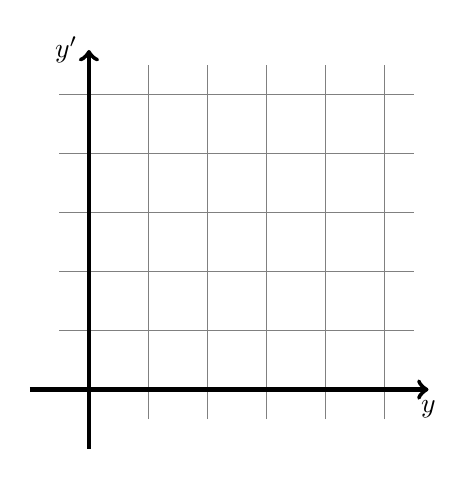
\begin{tikzpicture}[scale=0.75]
\draw[help lines] (-.5,-.5) grid (5.5, 5.5);
\draw[ultra thick, ->] (-1, 0) -- (5.75, 0) node[below] {$y$};;
\draw[ultra thick, ->] (0, -1) -- (0, 5.75) node[left] {$y'$};
\end{tikzpicture}
\end{center}
\end{questions}

\end{document}
